\chapter{Problem Statement}
\section{Statement}

The problem statement can be reduced to the following.
\begin{figure}[htpb]
\centering
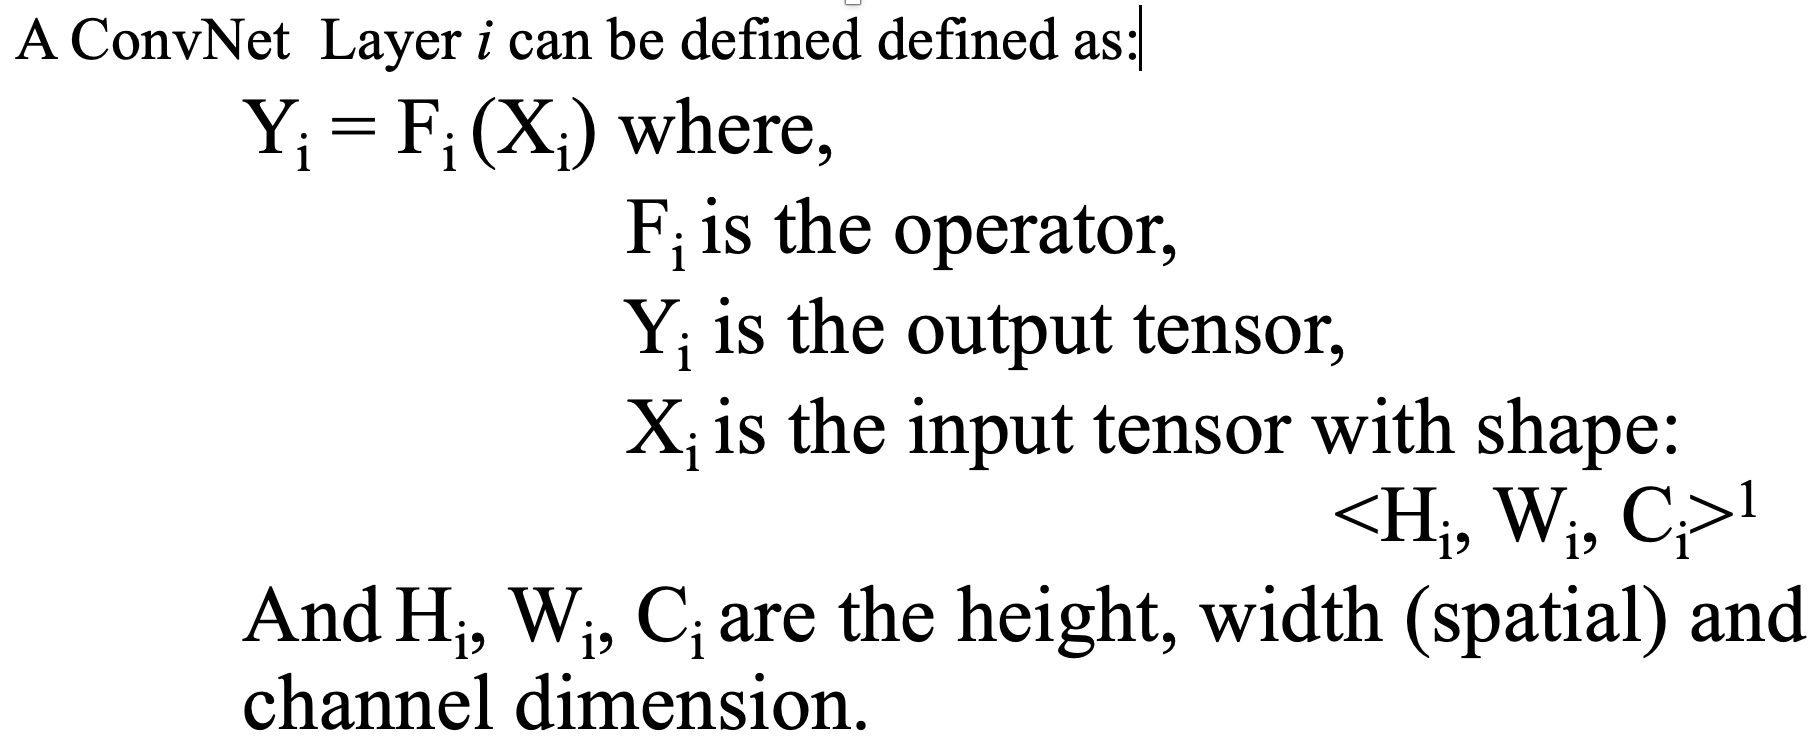
\includegraphics[width=\textwidth,height=\textheight,keepaspectratio]{../../static/Problem Definition.png}
\caption{Problem Definition.png}
\end{figure}The ConvNet can also be demonstrated as a series of layers, with the following form. In practice, ConvNet layers are often partitioned into multiple stages and all layers in each stage share the same architecture: for example, ResNet has five stages, and all layers in each stage has the same convolutional type except the first layer performs down-sampling. Therefore, we can define a ConvNet as:

\begin{figure}[htpb]
\centering
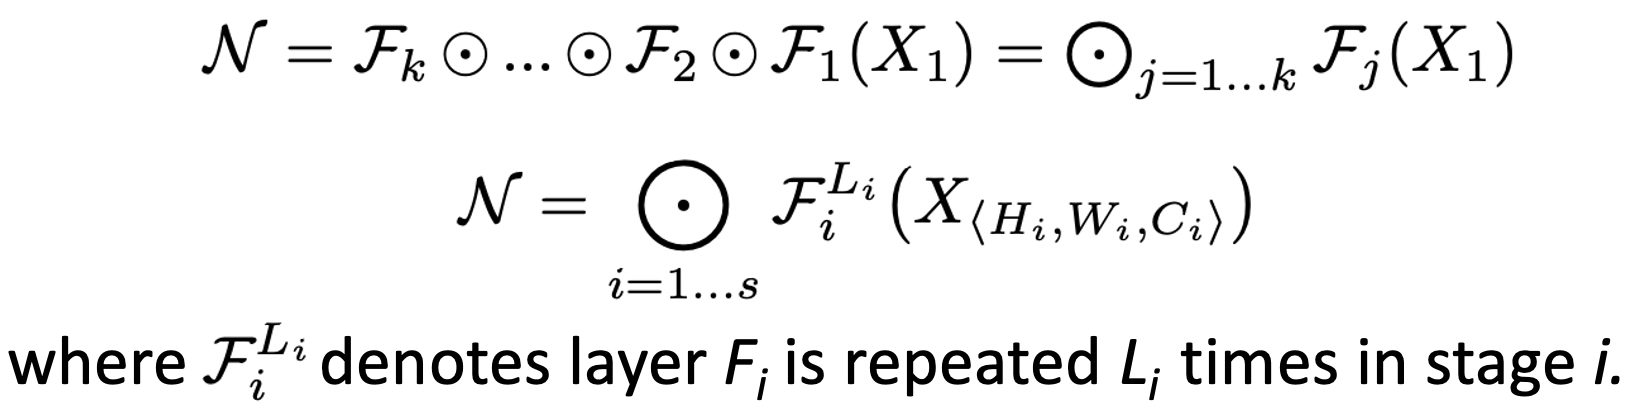
\includegraphics[width=\textwidth,height=\textheight,keepaspectratio]{../../static/Layer-wise representation of CNN.png}
\caption{Layer-wise representation of CNN.png}
\end{figure}Unlike regular model scaling, this method tries expand network length(Li), width(Ci), and/or resolution(Hi, Wi) without changing Fi. By fixing Fi, task of model scaling is simplified but there still remains a large design space to explore Li, Ci, Wi, Hi, for each layer. In order to further reduce design space, the authors restrict that all layers must be scaled uniformly with constant ratio. Hence the target is to maximize model accuracy for any given resource constraint, which can be formulated as the following optimization problem.




\begin{figure}[htpb]
\centering
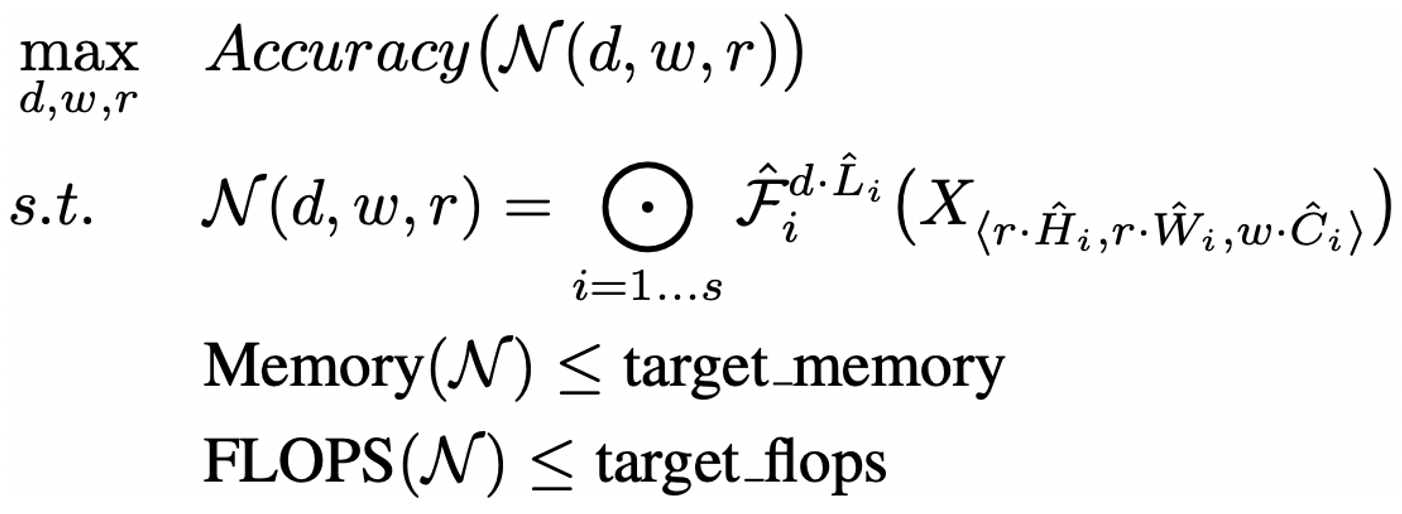
\includegraphics[width=\textwidth,height=\textheight,keepaspectratio]{../../static/Optimization Problem.png}
\caption{Optimization Problem.png}
\end{figure}